\section{Generación automática de código ST}

\begin{frame}{Generación automática de código ST}
  \begin{block}{Herramienta: Simulink PLC Coder}
    Traduce automáticamente los Statecharts a \textbf{Texto Estructurado} (ST, norma IEC 61131-3).
  \end{block}

  \begin{block}{Estructura del código generado}
    Autómata \textbf{plano y monolítico}: un \texttt{CASE} global sobre la variable de estado, con
    una densa red de \texttt{IF/ELSIF} anidados para resolver transiciones y acciones.
  \end{block}

  \begin{alertblock}{Manual (SFC) vs. autogenerado (ST)}
    \begin{itemize}
      \item \textbf{Eficiencia / CPU}: comparable (el compilador del PLC optimiza ambos).
      \item \textbf{Legibilidad y diagnóstico}: el ST autogenerado \textbf{carece de trazabilidad
            visual} $\Rightarrow$ difícil de interpretar en planta.
    \end{itemize}
    Por eso se optó por \textbf{SFC manual} para la arquitectura y ST sólo para los cálculos.
  \end{alertblock}
\end{frame}

\begin{frame}{Fragmento de código ST autogenerado (PLC Coder)}
  \centering
  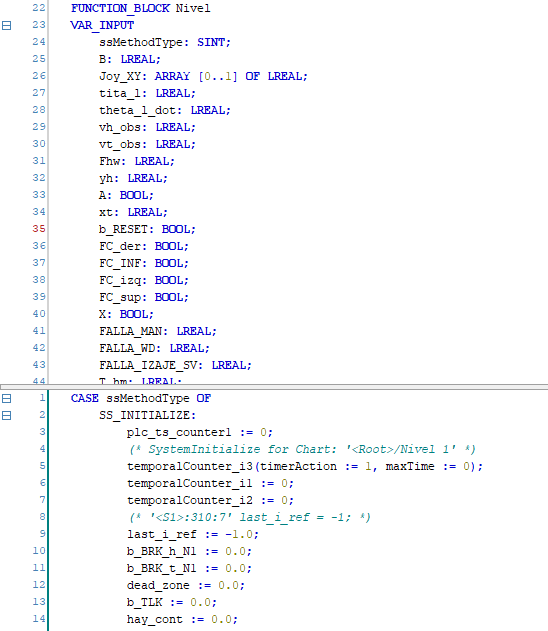
\includegraphics[width=\linewidth,height=0.82\textheight,keepaspectratio]{codesys/st_generado.png}
\end{frame}
